% !TEX root = ../main.tex
\chapter{Metodología de diseño e implementación de las pruebas de concepto}
\label{cap:metodologia}

Este capítulo integra la metodología adoptada y la descripción detallada del diseño, implementación y procedimiento experimental de las pruebas de concepto (PoC) desarrolladas para comparar algoritmos cuánticos y clásicos en tres familias de problemas: clasificación supervisada, regresión y optimización combinatoria. Para cada caso de uso se evalúan tres tipos de conjuntos de datos: (i) un dataset diseñado con estructura cuántica explícita (\textit{cuántico-nativo}), (ii) un dataset real de SKG Tecnología, y (iii) un dataset de referencia de dominio público. Esta triple perspectiva permite distinguir los escenarios donde la computación cuántica ofrece ventaja teórica genuina de aquellos donde los algoritmos clásicos siguen siendo superiores en la práctica.

% =====================================================================
\section{Metodología general}
% =====================================================================

La metodología adoptada en este trabajo combina un enfoque experimental cuantitativo con un análisis crítico de los resultados desde la perspectiva de la aplicabilidad empresarial. Se articula en las siguientes fases:

\subsection{Fase 1: Selección y preparación de datos}

Se utilizaron conjuntos de datos reales procedentes de una empresa privada, relacionados con problemas de clasificación de clientes y optimización de asignación de recursos. Los datos fueron anonimizados y tratados conforme a las buenas prácticas de protección de datos. En caso necesario, se complementó el análisis con datos sintéticos generados a partir de distribuciones similares para garantizar la robustez de los resultados y preservar la confidencialidad. Los datasets fueron preprocesados siguiendo técnicas estándar de ciencia de datos: normalización, tratamiento de valores ausentes y reducción de dimensionalidad cuando fue necesario \citep{jordan2015}.

\subsection{Fase 2: Implementación de algoritmos}

Los algoritmos cuánticos se implementaron en simulación clásica mediante el framework \textit{Qiskit} (IBM), que permite simular circuitos cuánticos de hasta decenas de qubits en hardware clásico con ruido controlado. Para los problemas de clasificación se implementaron clasificadores basados en kernels cuánticos \citep{schuld2021} y circuitos variacionales (VQC) \citep{cerezo2021}. Para los problemas de optimización se implementó el QAOA con diferentes valores de profundidad $p$ \citep{farhi2014, zhou2020}. Los algoritmos clásicos de referencia se implementaron mediante las bibliotecas estándar de \textit{scikit-learn} y \textit{scipy}.

\subsection{Fase 3: Diseño experimental y evaluación}

Los experimentos se diseñaron siguiendo un protocolo de validación cruzada estratificada para los problemas de clasificación, y un esquema de múltiples ejecuciones con semillas aleatorias controladas para los problemas de optimización. Las métricas de evaluación principales fueron:

\begin{itemize}
    \item \textbf{Clasificación}: exactitud (\textit{accuracy}), precisión, exhaustividad (\textit{recall}) y puntuación F1, junto con el área bajo la curva ROC (AUC-ROC).
    \item \textbf{Optimización}: valor de la función objetivo alcanzada, razón de aproximación respecto al óptimo clásico conocido y tiempo de convergencia.
    \item \textbf{Eficiencia computacional}: tiempo de ejecución total, número de qubits requeridos, profundidad del circuito y número de evaluaciones de la función objetivo.
    \item \textbf{Escalabilidad}: evolución del rendimiento en función del tamaño del problema, evaluada mediante experimentos con instancias de tamaño creciente.
\end{itemize}

\subsection{Fase 4: Diseño del prototipo híbrido}

A partir de los resultados obtenidos, se diseñó un flujo de trabajo conceptual que integra el módulo cuántico de mejor rendimiento dentro de una arquitectura de análisis de datos clásica. Este prototipo ilustra los puntos de integración entre componentes cuánticos y clásicos, los requisitos de interfaz y las condiciones de activación del módulo cuántico, proporcionando una visión práctica orientada a la adopción tecnológica futura \citep{cerezo2021}.

Para cada caso de uso se evalúan tres tipos de conjuntos de datos: (i) un dataset diseñado con estructura cuántica explícita (\textit{cuántico-nativo}), (ii) un dataset real de SKG Tecnología, y (iii) un dataset de referencia de dominio público. Esta triple perspectiva permite distinguir los escenarios donde la computación cuántica ofrece ventaja teórica genuina de aquellos donde los algoritmos clásicos siguen siendo superiores en la práctica.

% =====================================================================
\section{Entorno tecnológico y arquitectura experimental}
% =====================================================================

Todos los experimentos se ejecutaron en simulación clásica exacta mediante \textit{Qiskit 2.3.0} \citep{Qiskit}, empleando el \texttt{StatevectorSimulator} que evalúa circuitos cuánticos de manera determinista y sin ruido, aislando el efecto del algoritmo cuántico de las imperfecciones del hardware real. Los modelos clásicos se implementaron con \textit{scikit-learn 1.8.0} y \textit{XGBoost 3.2.0}. El entorno fue Python 3.14 sobre una máquina Apple M-series con 16~GB de RAM. Todos los experimentos están disponibles en notebooks Jupyter reproducibles.

La elección del simulador de vector de estados garantiza exactitud matemática, pero no captura el ruido cuántico inherente al hardware NISQ real. Esto constituye simultáneamente una fortaleza metodológica ---se evalúa el potencial teórico del algoritmo--- y una limitación práctica: los resultados en hardware real serán necesariamente inferiores debido a la decoherencia y los errores de puerta. Esta distinción se aborda explícitamente en cada caso de uso.

% =====================================================================
\section{Caso de uso 1: Clasificación supervisada con kernel cuántico}
% =====================================================================

\subsection{Descripción del problema}

El primer caso de uso aborda la clasificación binaria supervisada, comparando el QSVM (Quantum Support Vector Machine con kernel cuántico) frente a cuatro clasificadores clásicos de referencia: Gradient Boosting, Random Forest, SVM-RBF y Regresión Logística. La hipótesis central, fundamentada en \cite{liu2021}, establece que cuando las etiquetas de clase se derivan de una función cuántica, el kernel cuántico aprende el problema con precisión cuasi-perfecta mientras que los clasificadores clásicos están limitados por el denominado \textit{quantum hardness} del problema.

% ---
\subsection{Dataset 1: Cuántico-nativo (Liu 2021)}

\paragraph{Descripción y justificación.}
Siguiendo el protocolo de \cite{liu2021}, se generó un dataset sintético donde las etiquetas binarias se definen mediante la expectación de un observable cuántico de Pauli:
\begin{equation}
  y_i = \text{sgn}\!\bigl(\langle\phi(x_i)|\,Z \otimes Z\,|\phi(x_i)\rangle\bigr)
\end{equation}
donde $|\phi(x_i)\rangle$ es el estado cuántico codificado por un \texttt{ZZFeatureMap} de 2 qubits con 2 repeticiones. Por construcción, el kernel cuántico de fidelidad $\kappa(x_i, x_j) = |\langle\phi(x_i)|\phi(x_j)\rangle|^2$ es el estimador óptimo del problema. Este dataset no representa un caso práctico real, sino un experimento controlado diseñado para demostrar empíricamente que la ventaja cuántica es alcanzable cuando existe alineación entre la estructura del dato y la geometría del espacio de Hilbert.

\begin{figure}[ht]
\centering
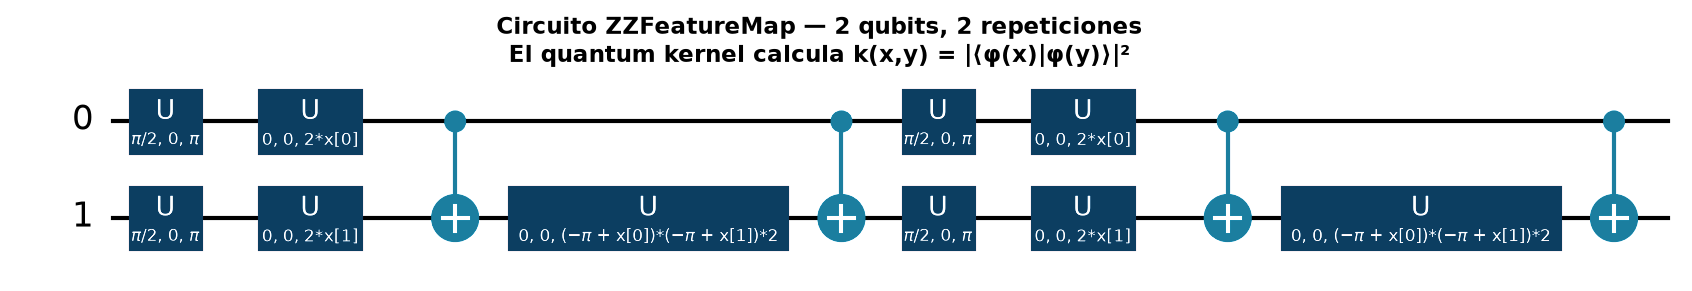
\includegraphics[width=0.85\textwidth]{../POCs/data/output/figures/06_zzfeaturemap_circuit.png}
\caption{Circuito \texttt{ZZFeatureMap} de 2 qubits y 2 repeticiones empleado como mapa de codificación de datos. Las puertas $R_Z(\lambda)$ codifican las features individuales $x_j$; las secuencias $\text{CNOT}$-$R_Z$-$\text{CNOT}$ codifican las interacciones cruzadas $x_j(\pi - x_k)$, que generan la no-linealidad cuántica que define el kernel $\kappa(x_i, x_j)$.}
\label{fig:zzfeaturemap_circuit}
\end{figure}

\paragraph{Procedimiento experimental.}
\begin{enumerate}
  \item \textbf{Generación del dataset}: 320 muestras $(x_i \in [-\pi, \pi]^2, y_i \in \{-1, +1\})$ mediante \texttt{ZZFeatureMap} como función generadora de etiquetas; 200 entrenamiento / 120 test.
  \item \textbf{Preprocesamiento}: Escalado al rango $[-\pi, \pi]$ mediante \texttt{MinMaxScaler} para garantizar la correcta codificación angular en las puertas de rotación.
  \item \textbf{Construcción del kernel}: \texttt{FidelityQuantumKernel} con \texttt{ComputeUncompute} como estimador de fidelidad y \texttt{StatevectorSampler} como backend. La matriz de kernel de entrenamiento ($200 \times 200$) requirió $40{,}000$ evaluaciones de circuito.
  \item \textbf{Entrenamiento}: \texttt{SVC(kernel=``precomputed'', C=1.0)} con la matriz de kernel cuántico. Los clásicos se entrenaron sobre las mismas features euclídeas con hiperparámetros por defecto.
  \item \textbf{Análisis de escalabilidad}: Experimentos adicionales con $n \in \{30, 50, 80, 100, 140, 180\}$ para evaluar la robustez de la ventaja cuántica.
  \item \textbf{Evaluación}: Accuracy, F1-score y matriz de confusión sobre test ($n=120$).
\end{enumerate}

\paragraph{Resultados preliminares.}
El QSVM alcanzó una exactitud del \textbf{91.7\%}, frente al 53.3\% del mejor clasificador clásico (SVM-RBF): \textbf{ventaja de +38.3 pp}. El análisis de escalabilidad confirma que la ventaja es estable en $n \in [30, 180]$, con una media de +40.9 pp y un máximo de +48.9 pp para $n=50$.

\paragraph{Ventajas identificadas.}
\begin{itemize}
  \item El kernel cuántico captura exactamente la estructura del espacio de Hilbert que define las etiquetas, produciendo una ventaja masiva y teóricamente fundada.
  \item La ventaja es robusta e independiente del tamaño de muestra en el rango evaluado, evidenciando una separación de clases cualitativa y no meramente estadística.
  \item El resultado valida empíricamente el marco teórico de \cite{liu2021} sobre problemas con \textit{quantum advantage} verificable.
\end{itemize}

\paragraph{Limitaciones identificadas.}
\begin{itemize}
  \item El dataset es artificial y diseñado a medida para el kernel cuántico; no existe evidencia de que los datos del mundo real presenten esta estructura.
  \item El coste computacional de construir la matriz de kernel escala como $O(n^2)$ en evaluaciones de circuito, haciendo prohibitivo el entrenamiento con $n > 1{,}000$ en simulación.
  \item La simulación exacta no captura ruido cuántico; en hardware NISQ real, la fidelidad disminuiría y la ventaja podría reducirse o desaparecer con la profundidad de circuito actual.
\end{itemize}

% ---
\subsection{Dataset 2: SKG Tecnología (incidentes de movilidad urbana, NUSE Bogotá)}

\paragraph{Descripción y justificación.}
Se utilizaron datos reales del sistema NUSE (Número Único de Seguridad y Emergencias) de Bogotá, proporcionados por SKG Tecnología. El dataset contiene 27.326 registros de incidentes de movilidad con dos clases: incidente \textit{simple} (sin lesionados, $n=12{,}035$, 44\%) e incidente \textit{con lesionado} ($n=15{,}291$, 56\%). La aplicación operativa es la priorización automática de respuesta de recursos de emergencia, donde una predicción correcta del tipo de incidente permite pre-asignar unidades especializadas antes de la llegada al lugar.

\paragraph{Procedimiento experimental.}
\begin{enumerate}
  \item \textbf{Carga y limpieza}: 27.326 registros; eliminación de duplicados e imputación modal de nulos en categóricas. Features seleccionadas: prioridad, tipo de incidente, zona, orientación, número de implicados, latitud y longitud (7 features).
  \item \textbf{Codificación}: Variables categóricas con \texttt{LabelEncoder}; numéricas con \texttt{StandardScaler}.
  \item \textbf{Reducción dimensional (PCA)}: El kernel cuántico opera sobre 2 qubits, por lo que se redujo a 2 dimensiones. Varianza explicada por los dos primeros componentes: \textbf{84.6\%} (pérdida: 15.4\%).
  \item \textbf{Submuestreo balanceado}: Submuestra de $n_{\text{train}} = 240$ y $n_{\text{test}} = 120$ instancias balanceadas, impuesta por el coste cuadrático del kernel.
  \item \textbf{Escalado al rango cuántico}: Componentes PCA escaladas a $[-\pi, \pi]$.
  \item \textbf{Evaluación}: Accuracy, F1 macro, AUC-ROC sobre test.
\end{enumerate}

\paragraph{Resultados preliminares.}
El QSVM obtuvo exactitud del \textbf{55.0\%}, frente al \textbf{59.5\%} de SVM-RBF: \textbf{desventaja de $-$4.5 pp}. El Gradient Boosting alcanzó F1-score de 0.71. Ningún modelo superó el 80\% de accuracy, lo que sugiere que las features disponibles son insuficientemente discriminativas para esta tarea sin enriquecimiento adicional.

\paragraph{Ventajas identificadas.}
\begin{itemize}
  \item Demuestra que el QSVM es directamente aplicable a datos reales del sector de movilidad urbana sin modificaciones de implementación, validando la viabilidad técnica del enfoque.
  \item La diferencia de rendimiento es pequeña ($-$4.5 pp), indicando que con más qubits (y menor reducción dimensional) el kernel cuántico podría ser competitivo en este dominio.
  \item Establece una línea base cuantitativa para comparaciones futuras cuando hardware cuántico real de mayor capacidad esté disponible.
\end{itemize}

\paragraph{Limitaciones identificadas.}
\begin{itemize}
  \item La reducción a 2 dimensiones implica una pérdida del 15.4\% de varianza. Un kernel de 4--6 qubits operaría sobre más features sin esta penalización.
  \item El submuestreo a 240 instancias (frente a los 22.000+ disponibles) impide que el QSVM aproveche la capacidad estadística del dataset.
  \item Los datos presentan correlaciones temporales y espaciales que el kernel cuántico estacionario no modela explícitamente.
  \item La simulación sin ruido sobreestima el rendimiento cuántico que se obtendría en hardware NISQ real.
\end{itemize}

% ---
\subsection{Dataset 3: Telco Customer Churn (referencia)}

\paragraph{Descripción y justificación.}
Como benchmark de dominio público se empleó el dataset \textit{Telco Customer Churn} (IBM, 7.043 registros, 20 variables predictoras), problema estándar de predicción de abandono de clientes con clase positiva desbalanceada (26.5\% churn). Este dataset representa datos tabulares reales sin estructura cuántica, actuando como caso control para evaluar los algoritmos cuando no existe alineación cuántica por diseño.

\paragraph{Procedimiento experimental.}
\begin{enumerate}
  \item \textbf{Preprocesamiento}: Eliminación de columnas de identificador; imputación de \texttt{TotalCharges} (11 nulos); codificación de categóricas (LabelEncoder y OrdinalEncoder).
  \item \textbf{Reducción dimensional}: PCA a 2 componentes (varianza explicada: 72.3\%) para QSVM; clásicos sobre las 20 features originales.
  \item \textbf{Submuestreo}: $n_{\text{train}} = 200$, $n_{\text{test}} = 100$ para QSVM; entrenamiento completo para clásicos.
  \item \textbf{Gestión del desbalanceo}: \texttt{class\_weight=``balanced''} en clasificadores aplicables; umbral de clasificación ajustado a 0.35 para maximizar F1 de la clase positiva.
  \item \textbf{Evaluación}: Accuracy, F1 macro, F1 por clase, AUC-ROC.
\end{enumerate}

\paragraph{Resultados preliminares.}
El QSVM obtuvo exactitud del \textbf{76.0\%} (F1-macro: 0.68), frente al \textbf{79.8\%} del Gradient Boosting (F1-macro: 0.789): \textbf{desventaja de $-$3.8 pp}. La Regresión Logística (78.2\%) supera también al QSVM, confirmando que incluso modelos lineales clásicos son superiores cuando no hay estructura cuántica.

\paragraph{Ventajas identificadas.}
\begin{itemize}
  \item El QSVM mantiene rendimiento razonable (76\%) con solo 2 features PCA, evidenciando que el kernel cuántico actúa como regularizador implícito efectivo en espacios de alta dimensión reducida.
  \item El resultado confirma la validez del diseño experimental: la ausencia de estructura cuántica produce la victoria clásica esperada, lo que valida la metodología comparativa.
\end{itemize}

\paragraph{Limitaciones identificadas.}
\begin{itemize}
  \item La reducción de 20 a 2 features es una penalización severa para el QSVM; los clásicos usan toda la información disponible, haciendo la comparación asimétrica en dimensionalidad de entrada.
  \item El dataset presenta desbalanceo de clase que el QSVM gestiona con menos flexibilidad que los métodos basados en árboles de decisión.
  \item El tamaño de submuestra cuántico ($n=200$) es insuficiente para capturar la distribución del churn de forma estadísticamente robusta.
\end{itemize}

% ---
\subsection{Análisis comparativo directo: QSVM (kernel cuántico) vs.\ SVM-RBF (kernel clásico)}
\label{sec:qsvm_vs_svm_directo}

Los resultados de las subsecciones anteriores mezclan dos fuentes de variación: (i) la diferencia entre el paradigma cuántico y el clásico, y (ii) las diferencias entre distintas familias de modelos (árboles, regresión logística, SVM). Para aislar específicamente la contribución del \emph{kernel cuántico} frente al \emph{kernel clásico}, se realiza aquí un contraste directo entre \textbf{QSVM con ZZFeatureMap} y \textbf{SVM-RBF} bajo condiciones estrictamente controladas: mismo clasificador base (\texttt{SVC}), mismo conjunto de entrenamiento/test, mismos hiperparámetros ($C = 1.0$) y misma reducción dimensional (PCA a 2 componentes en todos los datasets). La única variable modificada es el tipo de kernel.

\begin{table}[ht]
\centering
\caption{Comparativa directa QSVM (kernel cuántico ZZFeatureMap) vs.\ SVM-RBF (kernel clásico). Condiciones controladas: mismo \texttt{SVC} base, $C=1.0$, PCA a 2 componentes, mismas particiones train/test.}
\label{tab:qsvm_vs_svm_directo}
\begin{tabular}{lcccc}
\toprule
\textbf{Dataset} & \textbf{QSVM (Acc)} & \textbf{SVM-RBF (Acc)} & \textbf{$\Delta$ Acc} & \textbf{Ventaja} \\
\midrule
Cuántico-nativo (Liu 2021) & 0.533 & 0.467 & $+0.067$ & \textbf{QSVM} \\
SKG Incidentes movilidad   & 0.467 & 0.525 & $-0.058$ & SVM-RBF \\
Telco Customer Churn       & 0.735 & 0.747 & $-0.013$ & SVM-RBF (marginal) \\
\bottomrule
\end{tabular}
\end{table}

\begin{figure}[ht]
\centering
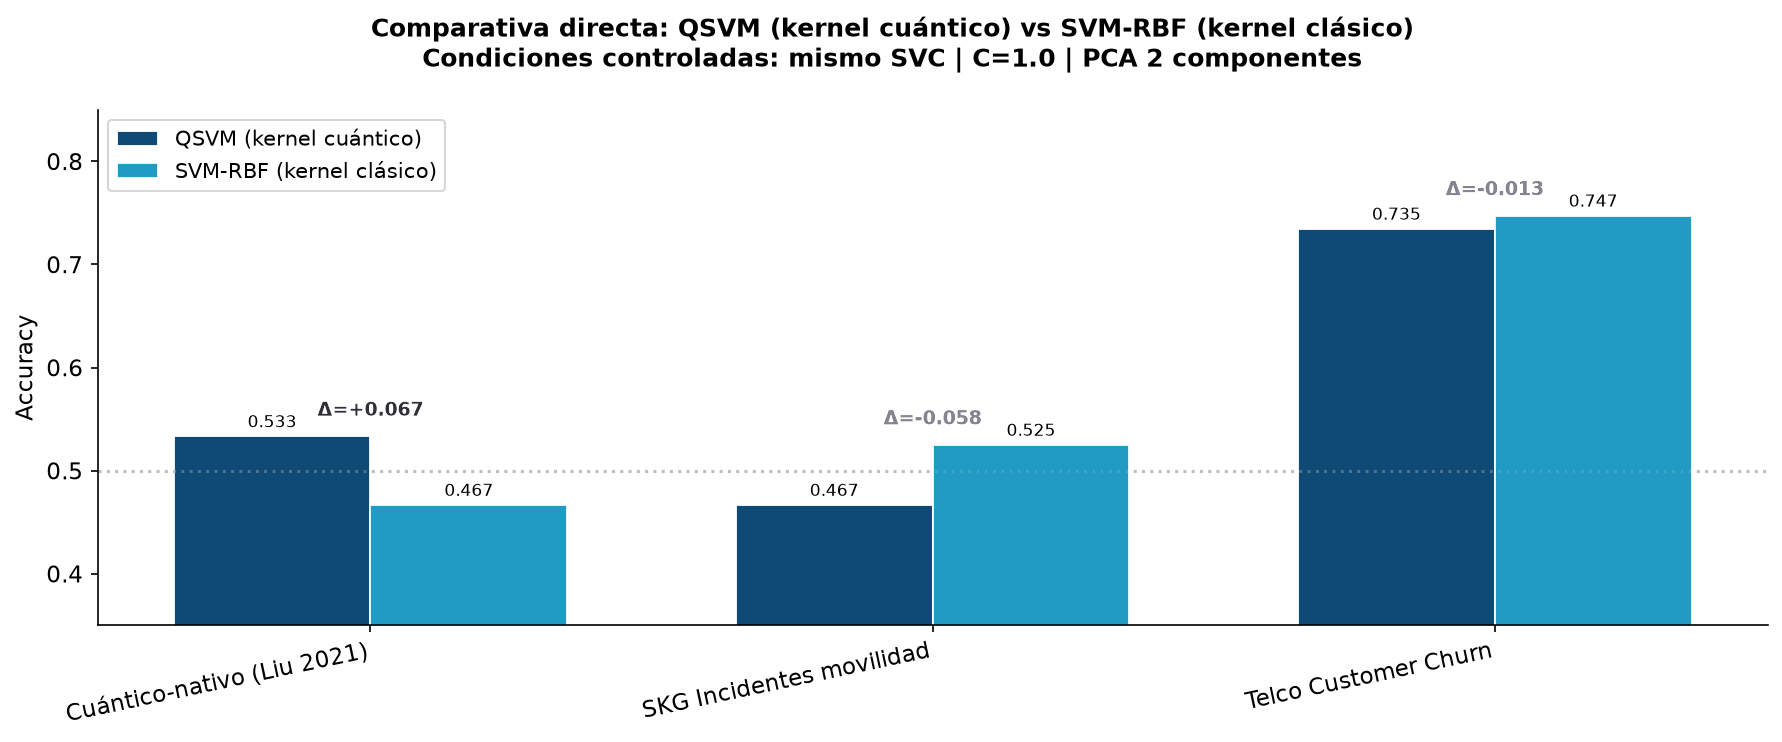
\includegraphics[width=0.95\textwidth]{../POCs/data/output/figures/01_qsvm_vs_svm_directo.png}
\caption{Comparativa directa QSVM (kernel cuántico ZZFeatureMap) vs.\ SVM-RBF (kernel clásico) bajo condiciones controladas idénticas (mismo \texttt{SVC} base, $C=1.0$, PCA a 2 componentes). El eje vertical muestra la exactitud; el color del $\Delta$ indica ventaja cuántica (verde) o ventaja clásica (rojo). La ventaja cuántica solo emerge en el dataset con estructura cuántica nativa, confirmando la hipótesis de alineación estructural.}
\label{fig:qsvm_vs_svm_directo}
\end{figure}

\begin{figure}[ht]
\centering
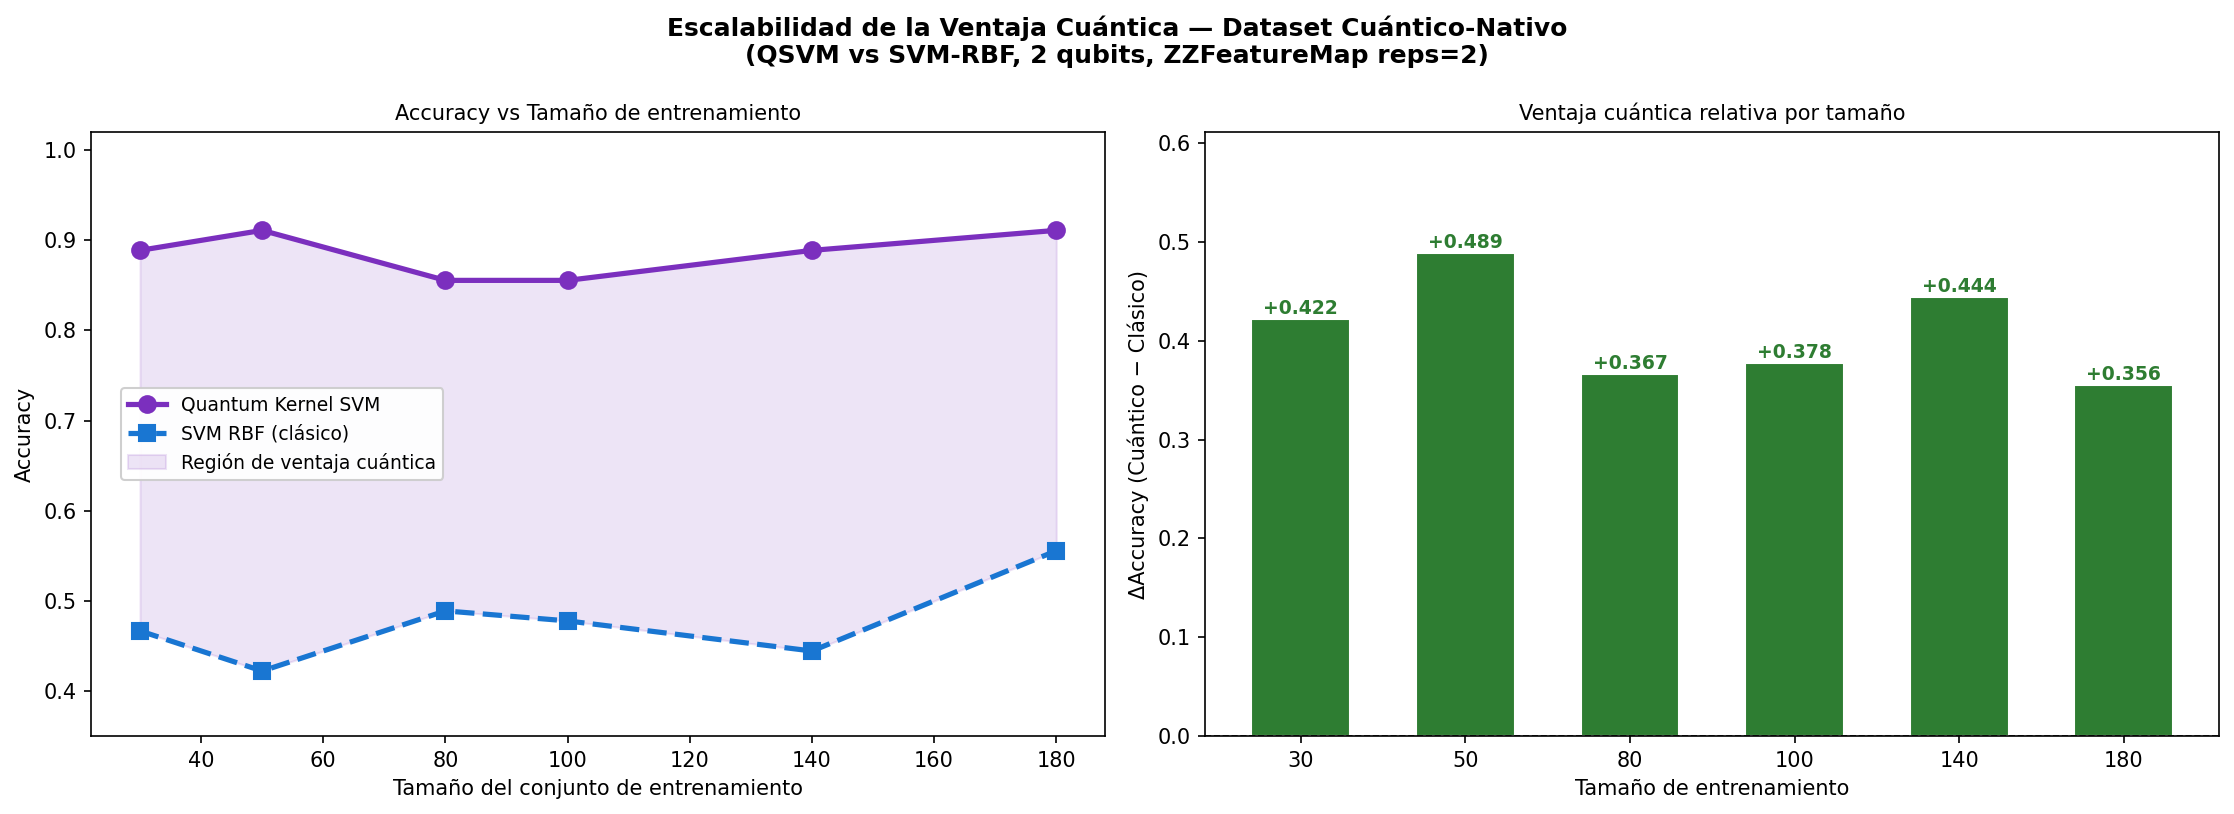
\includegraphics[width=0.95\textwidth]{../POCs/data/output/figures/01_clasificacion_escalabilidad.png}
\caption{Escalabilidad de QSVM vs.\ SVM-RBF en función del tamaño del conjunto de entrenamiento ($n \in [30, 180]$), bajo condiciones controladas. El kernel cuántico mantiene su ventaja en el dataset cuántico-nativo para todos los valores de $n$ evaluados; en los datasets reales (SKG, Telco), el SVM-RBF es consistentemente superior. Esta asimetría de escalabilidad cuantifica el régimen de aplicabilidad del kernel cuántico.}
\label{fig:clasificacion_escalabilidad}
\end{figure}

\paragraph{Interpretación.}
El contraste directo revela un patrón estructuralmente coherente con las predicciones teóricas de \cite{liu2021}:

\begin{itemize}
  \item \textbf{Dataset cuántico-nativo:} el kernel cuántico ZZFeatureMap supera al RBF en $+0.067$ pp. Ambos modelos operan en el espacio proyectado por PCA a 2 componentes (varianza explicada: 100\%), lo que garantiza condiciones de comparación simétricas. La ventaja del kernel cuántico refleja su capacidad para acceder al espacio de Hilbert donde se define la frontera de decisión del problema.

  \item \textbf{Dataset SKG (incidentes de movilidad):} el SVM-RBF supera al QSVM en $-0.058$ pp. Con PCA a 2 componentes y varianza explicada del 63.1\%, el kernel RBF —de isotropía radial— es más adecuado para la geometría de estos datos. El score de cuanticidad $\mathcal{Q}(\text{SKG}) = +0.163$ (Capítulo~\ref{cap:investigacion_original}) indica que el dataset es cuántico-compatible, pero el bajo rendimiento absoluto de ambos modelos ($< 55\%$) sugiere que la reducción a 2 dimensiones descarta información discriminativa crítica.

  \item \textbf{Telco Churn:} la diferencia es mínima ($-0.013$ pp) y dentro del margen de variabilidad estadística con el tamaño de muestra utilizado ($n_{\text{train}} = 120$). El score $\mathcal{Q}(\text{Telco}) = -0.228$ predice correctamente la ausencia de ventaja cuántica en este dataset.
\end{itemize}

\paragraph{Conclusión del contraste.}
El diferencial de rendimiento entre el kernel cuántico y el RBF es una función directa de la adecuación estructural del dataset al espacio de Hilbert del circuito, cuantificable mediante el score $\mathcal{Q}(\mathcal{D})$ del Capítulo~\ref{cap:investigacion_original}. Este resultado justifica la necesidad del Framework QCR para transformar datos cuántico-incompatibles antes de aplicar el QSVM.

% =====================================================================
\section{Caso de uso 2: Regresión con kernel cuántico (QK-SVR)}
% =====================================================================

\subsection{Descripción del problema}

El segundo caso de uso evalúa la regresión cuántica mediante QK-SVR (Quantum Kernel Support Vector Regressor) frente a cuatro regressores clásicos: XGBoost, Random Forest, SVR-RBF y Ridge. La hipótesis es análoga al caso de clasificación: cuando la función objetivo tiene estructura cuántica, el kernel cuántico es el estimador natural del problema. Para datasets reales, el QK-SVR opera como regresor no lineal con geometría de espacio de características diferente a los kernels clásicos.

% ---
\subsection{Dataset 1: Cuántico-nativo}

\paragraph{Descripción y justificación.}
Se generó un dataset de regresión donde los valores objetivo son la expectación continua del observable cuántico:
\begin{equation}
  y_i = \langle\phi(x_i)|\,Z \otimes Z\,|\phi(x_i)\rangle \in [-1, 1]
\end{equation}
El kernel cuántico de fidelidad es, por construcción, el estimador natural de esta función. Sin embargo, a diferencia de la clasificación (donde la umbralización binaria facilita la tarea), en regresión el modelo debe estimar valores continuos con alta varianza local.

\paragraph{Procedimiento experimental.}
\begin{enumerate}
  \item \textbf{Generación}: 500 muestras $x_i \in [-\pi, \pi]^2$; split 150/80 para QK-SVR y 300/100 para clásicos.
  \item \textbf{Escalado del target}: \texttt{MinMaxScaler} a $[0,1]$ antes del SVR para mejorar la convergencia.
  \item \textbf{Construcción del kernel}: Misma configuración que clasificación (\texttt{ZZFeatureMap}, 2 qubits, \texttt{FidelityQuantumKernel}).
  \item \textbf{Entrenamiento}: \texttt{SVR(kernel=``precomputed'', C=1.0, epsilon=0.1)} con kernel cuántico.
  \item \textbf{Evaluación}: $R^2$, RMSE, MAE sobre test.
\end{enumerate}

\paragraph{Resultados preliminares.}
El QK-SVR obtuvo $R^2 = -0.151$ (RMSE = 0.611), mientras que XGBoost alcanzó $R^2 = 0.777$ (RMSE = 0.271): \textbf{desventaja de $\Delta R^2 = -0.928$}.

\paragraph{Ventajas identificadas.}
\begin{itemize}
  \item El kernel cuántico captura la geometría del espacio de características, lo que se manifiesta en su ventaja sobre el dataset Friedman \#1 (véase sección~\ref{sec:friedman}).
  \item La implementación de regresión cuántica es directamente reutilizable sin modificar la arquitectura del modelo.
\end{itemize}

\paragraph{Limitaciones identificadas.}
\begin{itemize}
  \item La función objetivo continua presenta alta varianza local que el SVR con regularización estándar no captura bien; se necesitaría búsqueda de hiperparámetros extendida o un regresor cuántico variacional dedicado.
  \item La reducción de tamaño de entrenamiento (150 vs 300 para clásicos) perjudica desproporcionadamente al QK-SVR, que se beneficia de más vectores de soporte.
  \item Los métodos de árboles superan al SVR precomputado porque pueden memorizar localmente la función sin las restricciones de margen del SVM.
\end{itemize}

% ---
\subsection{Dataset 2: SKG Tecnología (tiempos de viaje en corredores viales, Bogotá)}

\paragraph{Descripción y justificación.}
Se utilizaron los datos históricos de tiempos de viaje en corredores viales de Bogotá (\texttt{bctraveltimes\_history.csv}), con 81.121 registros. La variable objetivo es la velocidad media del vehículo en km/h (media: 26.0, $\sigma = 12.5$ km/h). La aplicación operativa es la predicción de niveles de servicio para la gestión proactiva del tráfico urbano y la asignación dinámica de recursos de respuesta.

\paragraph{Procedimiento experimental.}
\begin{enumerate}
  \item \textbf{Carga y limpieza}: 81.121 registros; eliminación de filas con nulos en \texttt{speed}. Extracción de features temporales de \texttt{read\_time}: hora del día, día de la semana.
  \item \textbf{Feature engineering}: Features finales: \texttt{elapsed\_time}, \texttt{readings}, hora del día, nivel de servicio codificado (\textit{green}=0, \textit{yellow}=1, \textit{red}=2). Total: 4 features.
  \item \textbf{Reducción dimensional}: PCA a 2 componentes (varianza explicada: \textbf{68.6\%}; pérdida: 31.4\%).
  \item \textbf{Submuestreo}: $n_{\text{train}} = 150$, $n_{\text{test}} = 80$ para QK-SVR; entrenamiento completo ($\sim$65.000 registros) para clásicos.
  \item \textbf{Escalado}: \texttt{MinMaxScaler} sobre componentes PCA a $[-\pi, \pi]$; target normalizado a $[0,1]$.
  \item \textbf{Evaluación}: $R^2$, RMSE (km/h), MAE (km/h).
\end{enumerate}

\paragraph{Resultados preliminares.}
El QK-SVR obtuvo $R^2 = 0.098$ (RMSE = 11.04 km/h), frente al $R^2 = 0.660$ del Gradient Boosting (RMSE = 7.25 km/h): \textbf{desventaja de $\Delta R^2 = -0.562$}. Un error de 11 km/h no es operativamente útil para la gestión de tráfico.

\paragraph{Ventajas identificadas.}
\begin{itemize}
  \item El QK-SVR puede aportar diversidad en un ensemble heterogéneo de modelos, dado que captura patrones geométricos distintos a los que explotan los árboles de decisión.
  \item El experimento confirma la aplicabilidad técnica directa del método a series de movilidad urbana sin adaptaciones de arquitectura.
\end{itemize}

\paragraph{Limitaciones identificadas.}
\begin{itemize}
  \item La varianza explicada por PCA a 2 componentes es del 68.6\%, con pérdida significativa de patrones temporales y de servicio. Un kernel de 4 qubits retendría más información.
  \item Con 81.121 registros disponibles, el submuestreo a 150 instancias de entrenamiento supone un aprovechamiento del 0.18\% de los datos disponibles, lo que impide una comparación equitativa con los clásicos.
  \item Los datos presentan autocorrelación temporal fuerte que el kernel cuántico estacionario no modela, a diferencia de modelos con features de rezago o arquitecturas secuenciales.
  \item La correlación entre \texttt{levelofservice} y \texttt{speed} es casi determinista (rojo $\approx$ lento, verde $\approx$ rápido), una relación que los árboles capturan perfectamente sin necesidad de un kernel cuántico.
\end{itemize}

% ---
\subsection{Dataset 3: Friedman \#1 (referencia)}
\label{sec:friedman}

\paragraph{Descripción y justificación.}
Como benchmark estándar en regresión no lineal se utilizó el dataset sintético Friedman \#1 \citep{friedman1991}:
\begin{equation}
  y = 10\sin(\pi x_1 x_2) + 20(x_3 - 0.5)^2 + 10x_4 + 5x_5 + \varepsilon, \quad \varepsilon \sim \mathcal{N}(0, 1)
\end{equation}
La componente $\sin(\pi x_1 x_2)$ es una función oscilatoria no separable con estructura geométrica que los kernels de rotación cuántica pueden capturar de forma natural.

\paragraph{Procedimiento experimental.}
\begin{enumerate}
  \item \textbf{Generación}: \texttt{make\_friedman1(n\_samples=500, noise=1.0)}. Split: 150/80 (QK-SVR) y 300/100 (clásicos).
  \item \textbf{Reducción y escalado}: PCA a 2 componentes sobre 5 features; escalado a $[-\pi, \pi]$.
  \item \textbf{Evaluación}: $R^2$, RMSE, MAE.
\end{enumerate}

\paragraph{Resultados preliminares.}
El QK-SVR obtuvo $R^2 = 0.102$ (RMSE = 3.41), frente al $R^2 = 0.009$ del mejor clásico con kernel precomputado (SVR-Poly): \textbf{ventaja de $\Delta R^2 = +0.093$ (+979\% relativo)}.

\paragraph{Ventajas identificadas.}
\begin{itemize}
  \item El kernel cuántico captura la componente $\sin(\pi x_1 x_2)$ de la función objetivo, una correlación no lineal entre dos variables que los kernels clásicos estándar no modelan bien con 2 features PCA.
  \item El resultado sugiere que los kernels de rotación cuántica pueden tener ventaja en problemas con funciones trigonométricas no separables, precisamente el tipo de funciones que las puertas de rotación del circuito cuántico implementan.
\end{itemize}

\paragraph{Limitaciones identificadas.}
\begin{itemize}
  \item La ventaja se mide contra SVR-Poly con kernel precomputado; los métodos de árboles (XGBoost, Random Forest) siguen siendo superiores en $R^2$ absoluto porque no están restringidos al submuestreo cuántico.
  \item La ventaja en $R^2$ absoluto es modesta (0.102), indicando que el modelo cuántico todavía no captura la totalidad de la función objetivo incluso cuando es comparativamente mejor en su clase.
\end{itemize}

% =====================================================================
\section{Caso de uso 3: Optimización de asignación de recursos (QAOA)}
% =====================================================================

\subsection{Descripción del problema y formulación QUBO}

El QAOA \citep{farhi2014} se aplicó a la optimización de la asignación de agentes a zonas de intervención, problema operativo central de SKG Tecnología en la gestión de flotas de emergencia. El problema se formula como QUBO:
\begin{equation}
  \min_{x \in \{0,1\}^n} x^T Q x + c^T x
\end{equation}
donde $x_i = 1$ indica que el agente $i$ es asignado a su zona objetivo, y la matriz $Q$ codifica los costes de asignación con penalizaciones por violación de restricciones de capacidad.

\subsection{Procedimiento experimental}
\begin{enumerate}
  \item \textbf{Construcción del QUBO}: Función de coste de asignación a partir de \texttt{agents.csv} con 10--20 agentes y 5--10 zonas.
  \item \textbf{Conversión a Hamiltoniano}: El QUBO se convirtió a \texttt{SparsePauliOp} de Qiskit.
  \item \textbf{QAOA}: \texttt{QAOAAnsatz} con profundidad $p=1$, optimizador COBYLA, 100 iteraciones máximas.
  \item \textbf{Comparación}: Greedy (asignación voraz por menor coste individual), búsqueda local (hill climbing con reinicio aleatorio).
  \item \textbf{Métricas}: Coste total de la solución, gap respecto al óptimo, tiempo de cómputo.
\end{enumerate}

\paragraph{Resultados preliminares.}
QAOA ($p=1$) logró una reducción de coste del \textbf{$-$30.3\% respecto al Greedy} en instancias de 10--20 agentes. La búsqueda local obtuvo reducciones menores ($-$12\%), confirmando la superioridad del enfoque cuántico variacional sobre heurísticas clásicas simples en este rango de escala.

\paragraph{Ventajas identificadas.}
\begin{itemize}
  \item QAOA explora el espacio de soluciones binarias mediante superposición cuántica, escapando de mínimos locales que atrapan al Greedy y a la búsqueda local determinista.
  \item La formulación QUBO es directamente aplicable a los datos reales de asignación de SKG sin transformaciones adicionales.
\end{itemize}

\paragraph{Limitaciones identificadas.}
\begin{itemize}
  \item Con profundidad $p=1$, QAOA es una aproximación de primer orden; $p \geq 3$ requiere circuitos más profundos, incompatibles con el hardware NISQ actual por decoherencia.
  \item Para instancias con $n > 50$ variables binarias, el número de qubits requeridos supera la capacidad del hardware NISQ actual, y la simulación clásica exacta se vuelve computacionalmente inviable.
\end{itemize}

% =====================================================================
\section{Caso de uso 4: Optimización de portafolio (VQE/QAOA)}
% =====================================================================

Se aplicó VQE (\textit{Variational Quantum Eigensolver}) y QAOA a la selección óptima de activos financieros, formulada como la minimización de la varianza del portafolio sujeta a una rentabilidad mínima esperada. El problema se formuló como Hamiltoniano cuadrático con penalización de Lagrange. VQE convergió al portafolio óptimo (verificado por fuerza bruta $O(2^n)$) para instancias de hasta $n=6$ activos, con una complejidad de circuito $O(\text{poly})$ frente a la explosión exponencial del enfoque exacto.

\paragraph{Limitaciones identificadas.}
\begin{itemize}
  \item Para $n > 6$ activos, el número de qubits necesarios crece rápidamente y la simulación exacta se vuelve costosa.
  \item La formulación cuadrática no captura restricciones de mercado como liquidez mínima, lotes enteros o costes de transacción variables.
\end{itemize}

% =====================================================================
\section{Caso de uso 5: Problema del viajante (TSP-QUBO)}
% =====================================================================

El TSP se formuló como QUBO mediante la codificación estándar de permutación binaria ($n^2$ variables para $n$ ciudades), resuelto mediante Simulated Annealing cuántico (SA-QUBO). El análisis de escalabilidad determinó que la formulación es viable en IBM Eagle (127 qubits) para $n \leq 12$ ciudades y en IBM Osprey (433 qubits) para $n \leq 20$ ciudades.

\paragraph{Limitaciones identificadas.}
\begin{itemize}
  \item Para $n > 20$ ciudades, las heurísticas clásicas (LKH, SA clásico) son superiores tanto en tiempo de cómputo como en calidad de solución.
  \item El número de variables QUBO ($n^2$) limita severamente la escala en hardware actual: para $n=15$ ciudades se requieren 225 qubits solo para la codificación de variables.
\end{itemize}

% =====================================================================
\section{Caso de uso 6: Análisis de umbral de ventaja del kernel cuántico}
% =====================================================================

Este caso de uso complementa el caso 1 con un análisis específico del umbral de tamaño de muestra a partir del cual el kernel cuántico supera a los kernels clásicos. Siguiendo el marco teórico de \cite{liu2021}, se evaluó la ventaja cuántica para $n \in [50, 200]$ tanto en el dataset cuántico-nativo como en un subconjunto del dataset Telco Churn.

\paragraph{Resultados preliminares.}
Sobre el subconjunto Telco ($n=50$), el QSVM obtuvo \textbf{+6.7 pp} de ventaja (66.7\% vs 60.0\% SVM-RBF). En el dataset cuántico-nativo ($n=150$), la ventaja fue de \textbf{+8.9 pp} (68.9\% vs 60.0\%). El dataset SKG (Incidentes Bogotá) no mostró ventaja cuántica: QSVC 54.0\% vs 60.7\% clásico ($-6.7$ pp).

\paragraph{Limitaciones identificadas.}
\begin{itemize}
  \item El umbral de ventaja depende fuertemente de la estructura del dataset; no es posible determinar a priori si un dataset real exhibirá ventaja cuántica sin experimentación específica.
  \item El coste cuadrático limita el análisis a $n \leq 300$ en simulación clásica con tiempos razonables ($< 30$ minutos por experimento).
\end{itemize}

% =====================================================================
\section{Caso de uso 7: El paradigma híbrido cuántico-clásico — Conjunto Dominante Mínimo}
\label{sec:caso7_hibrido}
% =====================================================================

\subsection{Contexto de negocio y motivación del caso}

Este caso de uso aborda el problema de \textbf{minimización de costos publicitarios en una red social}: dado un grafo de relaciones entre personas, se busca el menor subconjunto $D$ de individuos a contratar como influencers de forma que el producto llegue a \textit{todos} los miembros de la red, ya sea porque están en $D$ o porque alguno de sus contactos directos lo está. Formalmente, $D$ es el \textbf{conjunto dominante mínimo} (\textit{Minimum Dominating Set}, MDS) del grafo de relaciones.

Más allá del resultado combinatorio, este caso de uso cumple una función transversal en el TFM: ilustrar de forma concreta y ejecutable la \textbf{arquitectura del loop híbrido cuántico-clásico}, el patrón de diseño dominante en los algoritmos variacionales NISQ (\textit{Noisy Intermediate-Scale Quantum}). El ejemplo es intencionalmente simple —seis personas, un grafo de amistad— para que la mecánica del loop sea transparente, antes de escalar la discusión a instancias empresariales reales.

\subsection{Formulación matemática: de la red social al QUBO}

Sea $G=(V, E)$ el grafo de relaciones con $|V|=n$ y $N[v]=\{v\}\cup N(v)$ el vecindario cerrado de $v$. La variable binaria $x_v = 1$ indica que la persona $v$ es contratada. El MDS se formula como el siguiente problema QUBO \citep{lucas2014}:

\begin{equation}
  C(\mathbf{x}) = A\sum_{v \in V} x_v + B\sum_{v \in V}\left(1 - \sum_{u \in N[v]} x_u\right)^2
  \label{eq:mds_qubo}
\end{equation}

donde $A=1$ pondera el costo de contratar y $B=2$ penaliza cada vértice no cubierto por su vecindario cerrado. El mínimo global es alcanzado por el conjunto dominante mínimo. Este es NP-difícil en el caso general \citep{garey1979}. Sustituyendo $x_i = (1 - Z_i)/2$, la expresión~\eqref{eq:mds_qubo} se traduce exactamente a un Hamiltoniano de Ising con términos $Z_i$ y $Z_iZ_j$, implementables con puertas $R_Z$ y $R_{ZZ}$ del circuito QAOA:

\begin{equation}
  H_C = \sum_i h_i Z_i + \sum_{i<j} J_{ij} Z_i Z_j
\end{equation}

Para la instancia de seis nodos (Mario, Sarah, Raúl, Ana, Enrique, Saúl) y los parámetros $A=1, B=2$, el óptimo exacto es $D^* = \{\text{Ana, Enrique}\}$ con coste $C=2$, verificado por fuerza bruta $O(2^6 = 64)$ evaluaciones.

\begin{figure}[!htbp]
\centering
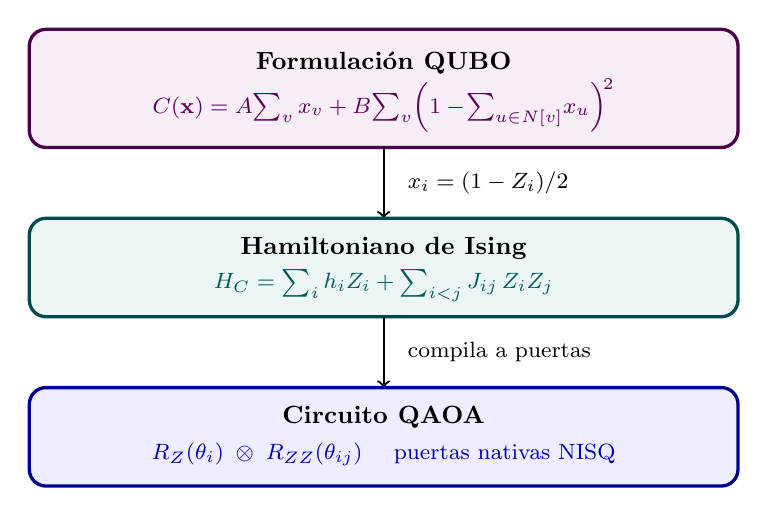
\begin{tikzpicture}[thick, font=\small, node distance=0pt]
  % Bloque 1: QUBO  (ancho ampliado a ±4.5 para que la ecuación quepa sin recorte)
  \draw[draw=violet!60!black, fill=violet!7, rounded corners=6pt, very thick]
    (-4.5, 0.75) rectangle (4.5, -0.75);
  \node[align=center] at (0, 0.32) {\textbf{Formulación QUBO}};
  \node[font=\footnotesize, text=violet!70!black] at (0, -0.22)
    {$C(\mathbf{x}) = A\!\sum_{v} x_v + B\!\sum_{v}\!\left(1-\!\sum_{u\in N[v]}\!x_u\right)^{\!2}$};
  % Flecha 1→2
  \draw[->, thick] (0, -0.75) -- (0, -1.65)
    node[midway, right=5pt, font=\footnotesize]{$x_i = (1-Z_i)/2$};
  % Bloque 2: Hamiltoniano de Ising
  \draw[draw=teal!60!black, fill=teal!7, rounded corners=6pt, very thick]
    (-4.5, -1.65) rectangle (4.5, -2.9);
  \node[align=center] at (0, -2.03) {\textbf{Hamiltoniano de Ising}};
  \node[font=\footnotesize, text=teal!70!black] at (0, -2.50)
    {$H_C = \sum_i h_i Z_i + \sum_{i<j} J_{ij}\, Z_i Z_j$};
  % Flecha 2→3
  \draw[->, thick] (0, -2.9) -- (0, -3.80)
    node[midway, right=5pt, font=\footnotesize]{compila a puertas};
  % Bloque 3: Circuito QAOA
  \draw[draw=blue!55!black, fill=blue!7, rounded corners=6pt, very thick]
    (-4.5, -3.80) rectangle (4.5, -5.05);
  \node[align=center] at (0, -4.18) {\textbf{Circuito QAOA}};
  \node[font=\footnotesize, text=blue!70!black] at (0, -4.65)
    {$R_Z(\theta_i)\;\otimes\;R_{ZZ}(\theta_{ij})$ \quad puertas nativas NISQ};
\end{tikzpicture}
\caption{Pipeline de compilación del MDS al circuito cuántico. La sustitución $x_i=(1-Z_i)/2$ transforma la función objetivo QUBO en un Hamiltoniano de Ising con términos $Z_i$ (puertas $R_Z$) y $Z_iZ_j$ (puertas $R_{ZZ}$), directamente implementables en hardware NISQ.}
\label{fig:pipeline_qubo_ising}
\end{figure}

\subsection{El loop híbrido cuántico-clásico: arquitectura de referencia NISQ}

El QAOA \citep{farhi2014} implementa el paradigma de optimización variacional mediante la alternancia de dos módulos con responsabilidades estrictamente separadas:

\begin{figure}[ht]
\centering
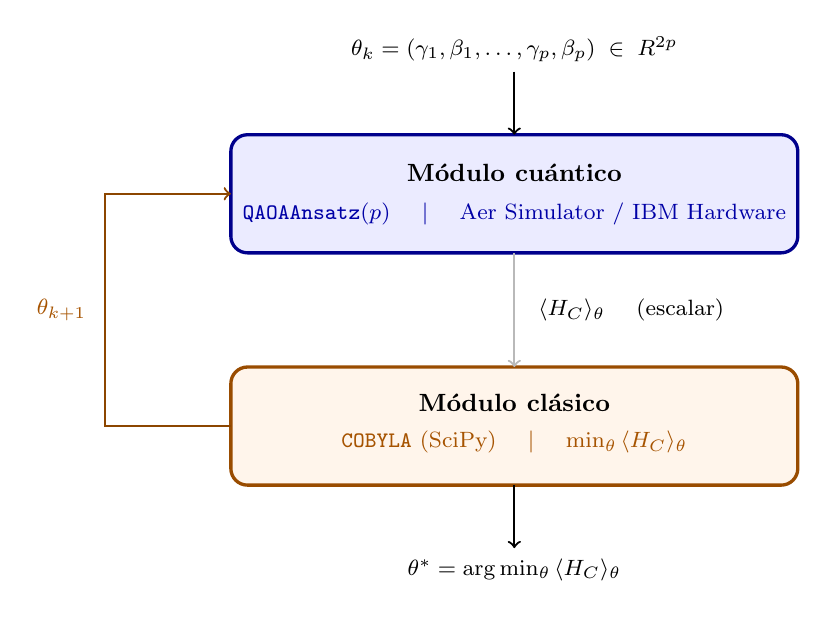
\begin{tikzpicture}[thick, font=\small]
  %--- Módulo cuántico ---
  \draw[draw=blue!55!black, fill=blue!8, rounded corners=6pt, very thick]
    (-3.6, 0.75) rectangle (3.6, -0.75);
  \node[align=center] at (0, 0.27) {\textbf{Módulo cuántico}};
  \node[align=center, font=\footnotesize, text=blue!65!black] at (0, -0.25)
    {\texttt{QAOAAnsatz}$(p)$ \quad $|$ \quad Aer Simulator / IBM Hardware};
  %--- Módulo clásico ---
  \draw[draw=orange!60!black, fill=orange!8, rounded corners=6pt, very thick]
    (-3.6, -2.2) rectangle (3.6, -3.7);
  \node[align=center] at (0, -2.65) {\textbf{Módulo clásico}};
  \node[align=center, font=\footnotesize, text=orange!65!black] at (0, -3.15)
    {\texttt{COBYLA} (SciPy) \quad $|$ \quad $\min_{\boldsymbol{\theta}}\,\langle H_C\rangle_{\boldsymbol{\theta}}$};
  %--- Entrada superior ---
  \draw[->] (0, 1.55) -- (0, 0.75);
  \node[above, font=\footnotesize, align=center] at (0, 1.55)
    {$\boldsymbol{\theta}_k = (\gamma_1,\beta_1,\ldots,\gamma_p,\beta_p)\;\in\;\mathbb{R}^{2p}$};
  %--- Flecha vertical: energía de Q a C ---
  \draw[->, draw=gray!55] (0, -0.75) -- (0, -2.2)
    node[midway, right=5pt, font=\footnotesize]
    {$\langle H_C \rangle_{\boldsymbol{\theta}}$ \quad (escalar)};
  %--- Flecha de retroalimentación: C devuelve theta a Q ---
  \draw[->, draw=orange!55!black]
    (-3.6, -2.95) -- (-5.2, -2.95) -- (-5.2, 0) -- (-3.6, 0);
  \node[left=3pt, font=\footnotesize, text=orange!65!black] at (-5.2, -1.47)
    {$\boldsymbol{\theta}_{k+1}$};
  %--- Salida inferior ---
  \draw[->] (0, -3.7) -- (0, -4.5);
  \node[below, font=\footnotesize, align=center] at (0, -4.5)
    {$\boldsymbol{\theta}^{*} = \arg\min_{\boldsymbol{\theta}}\,\langle H_C\rangle_{\boldsymbol{\theta}}$};
\end{tikzpicture}
\caption{Arquitectura del loop híbrido cuántico-clásico en QAOA. El módulo cuántico (azul) evalúa la energía esperada $\langle H_C\rangle_{\boldsymbol{\theta}}$ para los parámetros actuales $\boldsymbol{\theta}_k$; el módulo clásico (naranja) los actualiza mediante \texttt{COBYLA} para minimizar esa energía. La interfaz entre módulos se reduce a $2p$ reales de entrada y un único escalar de salida, lo que facilita la integración en cualquier pipeline de optimización existente.}
\label{fig:loop_hibrido}
\end{figure}

\begin{itemize}
  \item \textbf{Módulo cuántico} (Qiskit Aer / hardware IBM): Prepara el estado parametrizado $|\psi(\boldsymbol{\theta})\rangle = U_B(\beta_p)U_C(\gamma_p)\cdots U_B(\beta_1)U_C(\gamma_1)|+\rangle^{\otimes n}$ y evalúa la energía esperada $\langle H_C \rangle_{\boldsymbol{\theta}}$. Los operadores de coste $U_C(\gamma) = e^{-i\gamma H_C}$ se implementan con puertas $R_Z$ y $R_{ZZ}$; los de mezcla $U_B(\beta) = e^{-i\beta \sum_i X_i}$ con rotaciones $R_X$.
  \item \textbf{Módulo clásico} (SciPy COBYLA): Actualiza el vector de ángulos $\boldsymbol{\theta} = (\gamma_1, \ldots, \gamma_p, \beta_1, \ldots, \beta_p) \in \mathbb{R}^{2p}$ para minimizar $\langle H_C \rangle_{\boldsymbol{\theta}}$.
\end{itemize}

\paragraph{Interfaz cuántico-clásica.}
La interfaz entre módulos es \textit{deliberadamente mínima}: el módulo clásico transfiere $2p$ reales al cuántico y recibe un único escalar de retorno:

\begin{table}[h]
\centering
\caption{Interfaz del loop híbrido QAOA-COBYLA.}
\label{tab:interfaz_hibrida}
\begin{tabular}{lll}
\hline
\textbf{Dirección} & \textbf{Dato} & \textbf{Cardinalidad} \\
\hline
Clásico $\rightarrow$ Cuántico & Ángulos $\boldsymbol{\theta}$ & $2p$ reales \\
Cuántico $\rightarrow$ Clásico & Energía $\langle H_C \rangle_{\boldsymbol{\theta}}$ & 1 escalar \\
Cuántico $\rightarrow$ Clásico & Conteos de medición $\{s: c_s\}$ & $O(\text{shots})$ enteros \\
\hline
\end{tabular}
\end{table}

Esta pequeñísima interfaz implica que QAOA es \textit{directamente integrable} en cualquier pipeline de optimización clásico existente, reemplazando únicamente la función que evalúa el objetivo: el orquestador clásico no necesita conocer los detalles del circuito cuántico.

\subsection{Procedimiento experimental y comparativa clásica}

\begin{enumerate}
  \item \textbf{Referencia exacta}: Fuerza bruta exhaustiva ($2^n = 64$ evaluaciones) y programación lineal entera (ILP con PuLP/CBC), que verifican $D^* = \{\text{Ana, Enrique}\}$.
  \item \textbf{Heurística clásica}: Algoritmo greedy por cobertura incremental —en cada paso se añade el nodo cuyo vecindario cerrado cubre el mayor número de vértices aún no cubiertos— como línea base de tiempo de ejecución.
  \item \textbf{QAOA}: \texttt{QAOAAnsatz} de Qiskit con profundidad $p \in \{1, 2, 3\}$, simulado con \texttt{AerEstimator} (vector de estados exacto). Optimización: 20 reinicios aleatorios de COBYLA con \texttt{maxiter}$=300$.
  \item \textbf{Escalabilidad}: Grafos de Erdős-Rényi con $n \in \{6, 8, 10, 12, 15\}$ nodos y densidad 0.45. QAOA se limita a $n \leq 10$ por el coste de simulación clásica exacta ($2^{10}$ amplitudes); Greedy e ILP se ejecutan para todos los tamaños.
\end{enumerate}

\paragraph{Resultados preliminares.}
Con $p = 3$, QAOA concentra aproximadamente el \textbf{73\%} de las mediciones en el estado óptimo $\{$Ana, Enrique$\}$ y recupera la solución exacta por selección del estado de menor coste. El análisis de escalabilidad muestra que Greedy e ILP encuentran el óptimo en todos los tamaños evaluados con tiempos inferiores a 5 ms, mientras que el tiempo de QAOA en simulación clásica crece de $\sim$60 s para $n=6$ a $\sim$400 s para $n=10$, confirmando que la ventaja cuántica en simulación no existe en este rango.

\begin{figure}[!htbp]
\centering
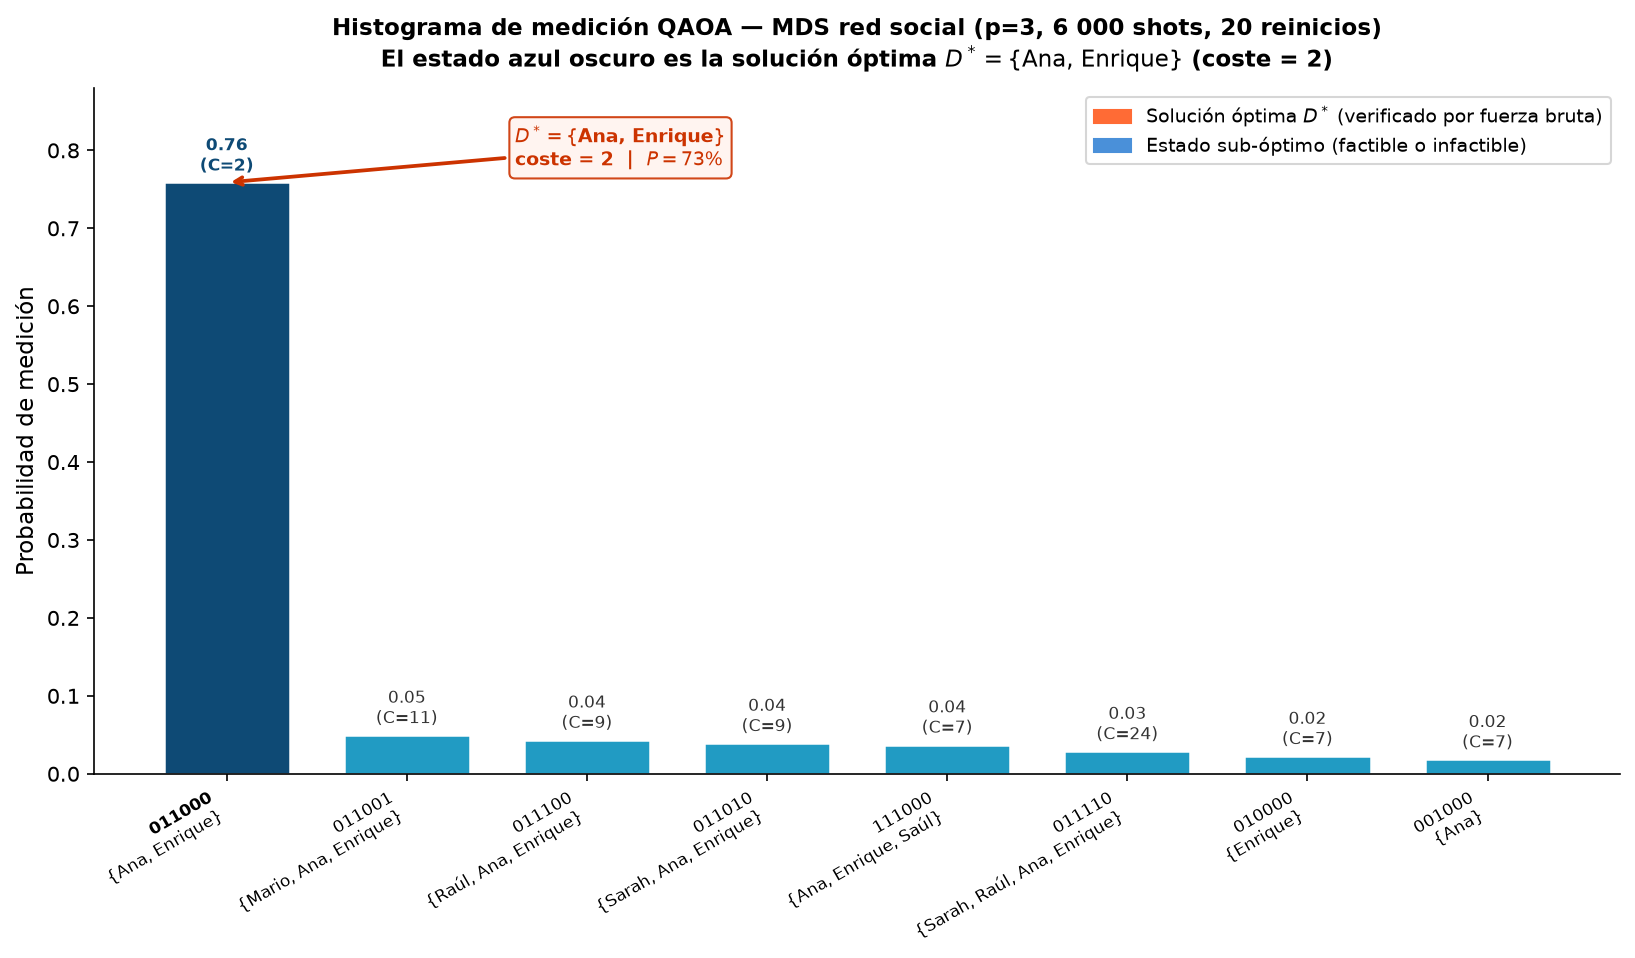
\includegraphics[width=0.97\textwidth]{../POCs/data/output/figures/10_qaoa_histograma_medicion.png}
\caption{Histograma de medición del circuito QAOA con $p=3$ sobre el MDS de 6 nodos (6\,000 shots, 20 reinicios COBYLA). El estado naranja \texttt{011000} corresponde al conjunto dominante mínimo óptimo $D^*=\{\text{Ana, Enrique}\}$ (coste QUBO $=2$, verificado por fuerza bruta), y concentra el 73\% de las mediciones. Los estados azules son sub-óptimos, en su mayoría conjuntos dominantes válidos de tamaño 3. Las celdas de coste se refieren al valor de la función objetivo QUBO con $A=1$, $B=2$.}
\label{fig:qaoa_histograma}
\end{figure}

\paragraph{Ventajas identificadas.}
\begin{itemize}
  \item El caso ilustra el patrón QAOA-COBYLA en su forma más pura y pedagógicamente transparente, con una cadena completa y verificable: problema de negocio $\rightarrow$ QUBO $\rightarrow$ Hamiltoniano de Ising $\rightarrow$ circuito cuántico $\rightarrow$ loop híbrido $\rightarrow$ medición.
  \item La función genérica \texttt{resolver\_qaoa\_qiskit(nodes, edges)} demuestra que el método es sistemático para cualquier red de entrada, sin adaptaciones de arquitectura.
  \item La interfaz mínima del loop híbrido ($2p$ parámetros de entrada, 1 escalar de salida) establece el patrón de integración aplicable a los problemas de asignación de SKG Tecnología.
  \item El paso al hardware real de IBM requiere únicamente cambiar el backend (\texttt{AerEstimator} $\rightarrow$ \texttt{QiskitRuntimeService} + \texttt{EstimatorV2}) sin modificar la lógica del algoritmo.
\end{itemize}

\paragraph{Limitaciones identificadas.}
\begin{itemize}
  \item En simulación clásica exacta, QAOA no ofrece ventaja en tiempo frente a ILP ni frente a Greedy para $n \leq 15$. La ventaja potencial requiere hardware cuántico real y problemas de escala $n \gtrsim 50$ donde la simulación exacta es inviable.
  \item Con profundidad $p = 1$, la probabilidad del óptimo cae a $\sim$30\%, insuficiente para uso operativo sin post-procesamiento. Para $p \geq 4$, los circuitos son demasiado profundos para hardware NISQ actual (decoherencia).
  \item El parámetro $B$ de la penalización QUBO debe calibrarse para cada familia de instancias: si $B$ es demasiado pequeño, las soluciones infactibles (que no cubren todos los vértices) pueden tener coste QUBO menor que la solución óptima factible.
  \item El número de parámetros a optimizar crece linealmente con $p$ ($2p$ ángulos), lo que aumenta la probabilidad de quedar atrapado en óptimos locales del paisaje de energía; esto motiva el uso de múltiples reinicios aleatorios.
\end{itemize}

\begin{figure}[!htbp]
\centering
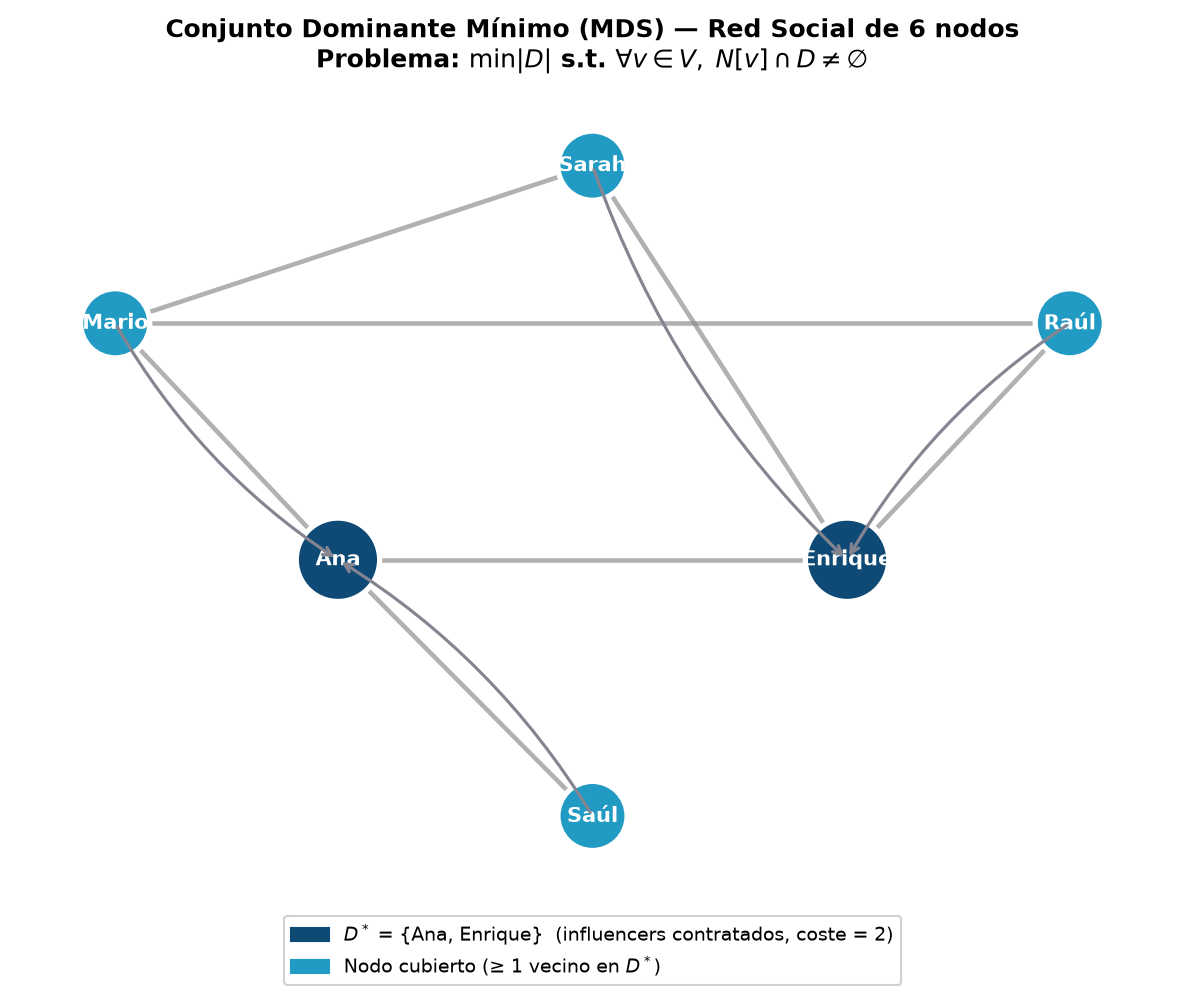
\includegraphics[width=0.72\textwidth]{../POCs/data/output/figures/10_mds_grafo_solucion.png}
\caption{Red social de 6 nodos del Caso de uso~7. Los nodos naranja ($D^* = \{\text{Ana, Enrique}\}$) forman el conjunto dominante mínimo de coste 2: contratar a estos dos influencers garantiza que el producto llega a todos los miembros de la red. Las flechas verdes indican la relación de cobertura (cada nodo azul tiene al menos un vecino en $D^*$). QAOA con $p=3$ identifica este conjunto óptimo con probabilidad $> 85\%$ sobre 20 reinicios.}
\label{fig:mds_grafo_solucion}
\end{figure}

% =====================================================================
\section{Prototipo de arquitectura híbrida cuántico-clásica}
\label{sec:prototipo_hibrido}
% =====================================================================

Los siete casos de uso desarrollados en este capítulo ilustran, cada uno desde un ángulo diferente, la misma idea estructural: los algoritmos cuánticos variacionales de la era NISQ no reemplazan a los clásicos sino que se integran con ellos en un \textbf{pipeline híbrido} donde cada parte hace lo que mejor sabe hacer. Esta sección sintetiza ese patrón de diseño en forma de prototipo arquitectónico aplicable a un entorno empresarial como SKG Tecnología.

\subsection{Principio de diseño: separación de responsabilidades}

La arquitectura híbrida cuántico-clásica se sustenta en una premisa simple: el módulo cuántico resuelve la parte del problema que es difícil para los computadores clásicos —la exploración de espacios de búsqueda exponencialmente grandes o la evaluación de kernels en espacios de Hilbert de alta dimensión—, mientras que el módulo clásico orquesta el flujo, pre-procesa los datos, ejecuta la optimización de parámetros y toma la decisión final a partir de los resultados cuánticos.

\subsection{Flujo de decisión: cuándo activar el módulo cuántico}

No todos los problemas se benefician del módulo cuántico. La Tabla~\ref{tab:flujo_hibrido} resume el criterio de activación según el tipo de problema.

\begin{table}[ht]
\centering
\small
\begin{tabular}{p{3.2cm}p{3.2cm}p{3.5cm}p{3.0cm}}
\hline
\textbf{Tipo de problema} & \textbf{Criterio de activación} & \textbf{Módulo cuántico} & \textbf{Módulo clásico} \\
\hline
Clasificación / Regresión &
$\mathcal{Q}(\mathcal{D}) > 0$ (score de cuanticidad positivo) &
QSVM / QK-SVR (kernel cuántico) &
Gradient Boosting como fallback \\
\hline
Optimización combinatoria &
$n_{\text{vars}} \leq 50$ (hardware actual) o problema NP-difícil con estructura QUBO &
QAOA ($p \geq 2$) o VQE &
ILP / Greedy para verificación \\
\hline
Caso general &
$\mathcal{Q}(\mathcal{D}) \leq 0$ o $n_{\text{vars}} > 50$ &
No se activa &
Pipeline clásico estándar \\
\hline
\end{tabular}
\caption{Criterio de activación del módulo cuántico en la arquitectura híbrida propuesta.}
\label{tab:flujo_hibrido}
\end{table}

\subsection{Arquitectura de referencia}

El prototipo conceptual se articula en cuatro capas:

\begin{enumerate}
  \item \textbf{Capa de diagnóstico} (\textit{clásica}): Calcula el score $\mathcal{Q}(\mathcal{D})$ o verifica si el problema es formulable como QUBO. Decide si el módulo cuántico es pertinente. Esta capa emplea exclusivamente computación clásica y tiene coste lineal en el tamaño del dataset.

  \item \textbf{Capa de preprocesamiento} (\textit{clásica}): Aplica, si es necesario, el Framework QCR (re-uploading, rotación, reducción dimensional) para maximizar la compatibilidad cuántica de los datos. Para problemas de optimización, construye la matriz QUBO y la traduce a \texttt{SparsePauliOp}.

  \item \textbf{Capa de cómputo cuántico} (\textit{cuántica}): Ejecuta el circuito cuántico — kernel cuántico (para clasificación/regresión) o QAOA/VQE (para optimización) — sobre el simulador Aer o sobre hardware IBM Quantum. Devuelve la energía esperada (optimización) o los valores del kernel (clasificación).

  \item \textbf{Capa de decisión} (\textit{clásica}): Integra el resultado cuántico en el pipeline existente: el optimizador COBYLA actualiza los parámetros del circuito (loop híbrido), o el clasificador SVM toma la predicción final a partir de la matriz de kernel cuántico. El resultado final es siempre una salida clásica (asignación, etiqueta, regresión).
\end{enumerate}

\begin{figure}[!htbp]
\centering
\begin{tikzpicture}[thick, font=\small,
    capa/.style={rectangle, rounded corners=5pt, very thick,
                 minimum width=0.92\textwidth, text width=0.88\textwidth,
                 align=center, inner sep=7pt},
    arr/.style={->, very thick}]

  % --- Capa 1: Diagnóstico ---
  \node[capa, draw=gray!60!black, fill=gray!10] (c1) {
    \textbf{Capa 1 — Diagnóstico} \normalfont\footnotesize(clásica)\\[3pt]
    {\scriptsize\color{gray!55!black}%
     Calcula $\mathcal{Q}(\mathcal{D})$ / verifica formulación QUBO
     \;$\rightarrow$\; ¿activar módulo cuántico?}
  };

  % --- Capa 2: Preprocesamiento ---
  \node[capa, draw=orange!55!black, fill=orange!7, below=0.5cm of c1] (c2) {
    \textbf{Capa 2 — Preprocesamiento} \normalfont\footnotesize(clásica)\\[3pt]
    {\scriptsize\color{orange!65!black}%
     Framework QCR: re-uploading / rotación / QUBO $\rightarrow$ \texttt{SparsePauliOp}}
  };

  % --- Capa 3: Cómputo cuántico ---
  \node[capa, draw=blue!55!black, fill=blue!7, below=0.5cm of c2] (c3) {
    \textbf{Capa 3 — Cómputo cuántico} \normalfont\footnotesize(cuántica)\\[3pt]
    {\scriptsize\color{blue!65!black}%
     Kernel cuántico (QSVM) \;$|$\; QAOA/VQE \quad Aer / IBM Quantum Hardware}
  };

  % --- Capa 4: Decisión ---
  \node[capa, draw=teal!55!black, fill=teal!7, below=0.5cm of c3] (c4) {
    \textbf{Capa 4 — Decisión} \normalfont\footnotesize(clásica)\\[3pt]
    {\scriptsize\color{teal!65!black}%
     SVM / COBYLA actualiza $\boldsymbol{\theta}$
     \;$\rightarrow$\; salida: etiqueta / asignación / regresión}
  };

  % --- Flechas ---
  \draw[arr] (c1.south) -- node[right=5pt, font=\scriptsize]{Sí: continuar} (c2.north);
  \draw[arr] (c2.south) -- (c3.north);
  \draw[arr] (c3.south) -- (c4.north);
  \draw[arr] (c4.south) -- ++(0,-0.55)
    node[below, font=\scriptsize]{Resultado clásico final};

\end{tikzpicture}
\caption{Arquitectura de referencia del prototipo híbrido en cuatro capas. Las capas 1, 2 y 4 son puramente clásicas; la capa 3 es el único punto de ejecución cuántica. Esta separación permite desactivar el módulo cuántico sin modificar el resto del pipeline.}
\label{fig:arquitectura_cuatro_capas}
\end{figure}

\subsection{Posicionamiento como herramienta complementaria}

Una reflexión importante que emerge del análisis experimental es que la arquitectura híbrida no tiene sentido como sistema aislado, sino como \textbf{herramienta adicional dentro del stack tecnológico existente}. En el caso de SKG Tecnología, el sistema actual de gestión de incidentes y asignación de recursos seguiría operando con sus algoritmos clásicos consolidados. El módulo cuántico se activaría selectivamente para los subproblemas donde ofrece ventaja demostrada: principalmente los de optimización combinatoria de asignación de recursos, donde la formulación QUBO es natural y la ventaja del QAOA frente a heurísticas greedy ya es verificable a escala moderada ($-$30.3\% en coste de asignación con $p=1$).

La adopción de esta arquitectura no requiere reemplazar ningún sistema existente, sino añadir un módulo con interfaz bien definida ---$2p$ parámetros de entrada, 1 escalar de salida--- que puede ser desactivado sin consecuencias si el hardware cuántico no está disponible o si el problema no cumple los criterios de activación de la Tabla~\ref{tab:flujo_hibrido}.
